\section{Electric Load Center Distribution Manager}\label{electric-load-center-distribution-manager}

\subsection{Overview}\label{overview-016}

The electric load center distribution manager (object name: ElectricLoadCenter:Distribution) is used organize power conversion devices and provides supervisory control over generators and storage.   Electric load centers can be thought of as subpanels connected to the facility's main electric panel.  Except for two applications for transformers that are located between the main panel and the utility grid connection, all other devices are associated with a specific load center.  The load center connects the “load” to the generators and “supply” power to the main panel serving the rest of the building.  A load center can have any number of generators but only one storage, (DC to AC) inverter, (AC to DC) converter or (isolation) transformer.  There are two separate operation schemes, one for generators and one for storage.  The generator operation scheme controls the on-site generators connected to a particular load center.  The storage operation scheme controls charging and discharging of electrical storage.  The generator operation is managed before the storage operation.  The internal meters used by EnergyPlus for reporting do all of the tracking. For more details on the individual inputs required see the Input Output Reference document.

The electric load center manager sums all of the building and system electric loads and provides operating schemes for the generators. The electric load center objects are operated in the order they are defined in the input data file (IDF), and generators are dispatched sequentially in the order they are specified within the list referenced by each load center object. The electricity produced from photovoltaic arrays and wind turbines is handled somewhat separately and is always run rather than being dispatched by supervisory control.  What is not provided by the on-site generation equipment, and electric storage units, is met by (purchasing) off-site electricity. It is possible to prescribe a set of ElectricLoadCenter:Distribution objects with inconsistent or conflicting operating schemes, so users need to be careful.

\subsection{Generator Operation Schemes}

The available generator operating schemes are “Baseload”, “DemandLimit”, “TrackElectrical,” “TrackSchedule,” “TrackMeter,” “FollowThermal” and “FollowThermalLimitElectrical.”  These operating schemes affect how loads are dispatched to the generators, in effect telling the generators whether or not to run and requesting power levels.

The Baseload scheme operates the generators at their rated (requested) electric power output when the generator is scheduled ON (ref. ElectricLoadCenter:Generators in the Input Output Reference). The Baseload scheme requests all generators scheduled ON (available) to operate, even if the amount of electric power generated exceeds the total facility electric power demand.

The DemandLimit scheme limits the amount of purchased electricity from the utility to the amount specified in the input. The Demand Limit scheme tries to have the generators meet all of the demand above the purchased electric limit defined by the user.

The TrackElectrical scheme tries to have the generators meet all of the electrical demand for the building.

The TrackMeter scheme tries to have the generators meet all the electrical demand from a meter chosen by the user rather than the usual meter for the entire facility. The meter can be a custom meter so that generators are tied to only certain loads in the building.

The TrackSchedule scheme tries to have the generators meet all of the electrical demand determined by a user-defined schedule.

The FollowThermal and FollowThermalLimitElectrical schemes run the generators to meet thermal demand. The thermal demand is determined from the plant modeling and depends on the flow requested by other components on the demand side of the plant loop, the loop temperatures, and the loop temperature setpoint. The electric load center distribution manager converts the thermal load to an electrical load using a nominal ratio of the thermal to electrical power production for each generator. For these schemes, the generator needs to be connected to the supply side of a plant loop and serve components that use hot water on the demand side of the plant loop. The thermal load request is obtained from the plant data structure (structure location in code is PlantLoop\%LoopSide\%Branch\%Comp\%MyLoad).The distribution manager converts the thermal load, $q_{thermal}$, to an electrical load using:

\begin{equation}
{q_{Elect}} = \frac{{{q_{thermal}}}}{{ThermElectRatio}}
\end{equation}

where,

$ThermElectRatio$\ is a nominal, constant, user-defined value for the ratio of thermal production to electrical production for a cogenerator. This ratio is used for supervisory control and dispatch of the electric power request to the generator; however, the cogenerator model may determine that actual performance varies from this nominal value at different times in the simulation when operating conditions differ from those used for the nominal ratio.

For all generator operating schemes except Baseload, a total electric load reduction target (or thermal load converted to electrical equivalent) is established for the load center based on the specific operating scheme. The load center then requests that its generators operate, one-by-one in the order specified in the generator list, until the target is met or exceeded. Generators that are not scheduled as ‘available’ for the simulation time step are not called to operate. The requested power demand to be met by each generator is the **smaller of** the nominal ‘rated’ electric power output (as specified in the ElectricLoadCenter:Generators object) or the remaining total electric load reduction target for the load center. After each electric generator is requested to operate, the actual electric power delivered by the generator, which may be greater than or less than the requested amount due to inputs specified in the generator performance model (e.g., Generator:CombustionTurbine, Generator:MicroTurbine, etc.), is used to update the remaining total electric power target for the other generators associated with this load center.

Most of the operating schemes will sequentially load the available electric load centers and generators. EnergyPlus can accept multiple “ElectricLoadCenter:Distribution” objects with different operating schemes. Because of this, there are two levels of reporting, one for the whole building and a second for each load center. The whole-building results are managed with the internal meters for the entire model. The individual load-center results are summed for those generators connected to a particular load center. The total electricity purchased is reported both in power and energy units. This value is positive when the amount of energy is purchased from the utility. This value can be negative when the total electricity produced is greater than the facility electrical needs. The excess will either be available for storage or to sell back to the electric utility company.

The order of input objects (ElectricLoadCenter:Distribution) in the input file is significant and used to structure how generators are dispatched with the first load centers and generators managed before the later ones. Therefore, load centers listed earlier in the file effectively have a higher priority.

\subsection{Load Center Buss Types}

Electric load centers can have one of five different configurations. Load centers can get fairly complicated and include power conditioning and storage. Separate inverter models are used to condition DC power from photovoltaics into AC power for the building and utility. The other generators may have inverters inside the devices but these are already embedded in the generator models. The load center can also supervise electrical storage controls and depend on the buss configuration. The transformer is optional for all buss types but if included in the load center it can be used to model an isolation or voltage matching transformer acting on the load center.

The most basic configuration is selected with the keyword “AlternatingCurrent” for the Electrical Buss Type, shown in the following diagram.

\begin{figure}[hbtp] % fig 333
\centering
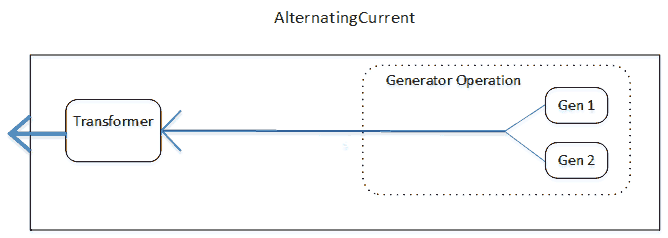
\includegraphics[width=0.9\textwidth, height=0.9\textheight, keepaspectratio=true]{media/ACBussDiagram.png}
\caption{Basic Alternating Current Schematic \protect \label{fig:basic-alternating-current-schematic}}
\end{figure}

The *AlternatingCurrent* load centers have AC generators with no storage and behave in the following way. All electric demand not met by the sum of the electrical power produced by the available generators will be met by purchased electricity.  If a generator is needed in the simulation for a small load and the load is less than the generator’s minimum part load ratio, the generator will operate at the minimum part load ratio and the excess will either reduce demand or the excess energy will be exported back to the electric utility company. 

A configuration with AC generators with on-site electrical storage is selected with the keyword “AlternatingCurrentWithStorage” and is shown in the following diagram. 

\begin{figure}[hbtp] % fig 334
\centering
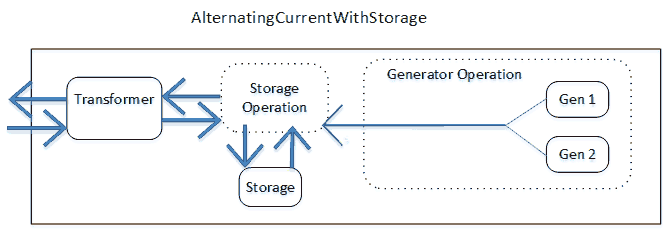
\includegraphics[width=0.9\textwidth, height=0.9\textheight, keepaspectratio=true]{media/ACStorageBussDiagram.png}
\caption{AC Generators with On-site Electrical Storage Schematic \protect \label{fig:ac-generators-with-on-site-electrical-storage}}
\end{figure}

The *AlternatingCurrentWithStorage* load centers attempt to augment the generator electricity production so that the power requests are met. Storage control logic is discussed below under Storage Operation Scheme.

The basic configuration for photovoltaic generators is selected using the “DirectCurrentWithInverter” keyword and is shown in the following diagram.

\begin{figure}[hbtp] % fig 335
\centering
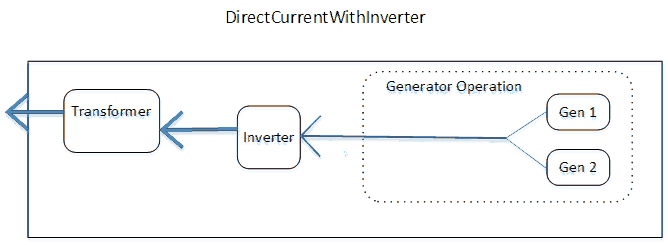
\includegraphics[width=0.9\textwidth, height=0.9\textheight, keepaspectratio=true]{media/DCInverterBussDiagram.png}
\caption{Direct Current With Inverter Photovoltaic Generators Schematic \protect \label{fig:direct-current-with-inverter-photovoltaic}}
\end{figure}

The *DirectCurrentWithInverter* load centers collect DC power from various generators, usually PV arrays, run the DC power through an inverter and produce AC power. The PV arrays produce DC power based on the availability of sunshine and do not respond to load requests made by the electric load center. 

If the PV-based load center is equipped with DC electrical storage that is connected before the inverter, then the buss type should be “DirectCurrentWithInverterDCStorage” and is shown in the following diagram.

\begin{figure}[hbtp] % fig 336
\centering
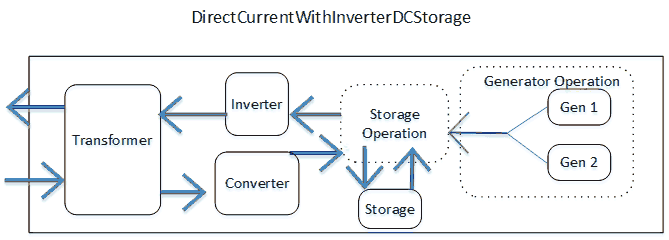
\includegraphics[width=0.9\textwidth, height=0.9\textheight, keepaspectratio=true]{media/DCInverterWithDCStorageBussDiagram.png}
\caption{PV based Load Center with DC Electrical Storage Schematic \protect \label{fig:pv-based-load-center-with-dc-electrical}}
\end{figure}

The *DirectCurrentWithInverterDCStorage* load centers charge or draw DC power to meet the requested electrical load depending on the storage operation scheme.

If the PV-based load center is equipped with AC electrical storage that is connected after the inverter, then the buss type should be “DirectCurrentWithInverterACStorage” and is shown in the following diagram.

\begin{figure}[hbtp] % fig 337
\centering
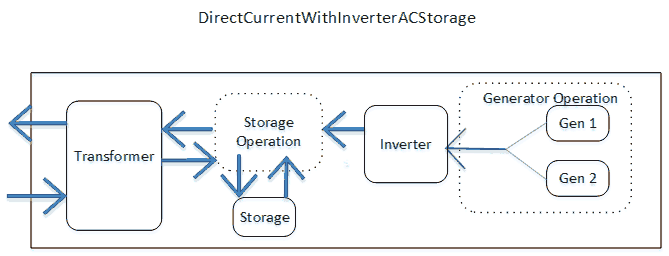
\includegraphics[width=0.9\textwidth, height=0.9\textheight, keepaspectratio=true]{media/DCInverterWithACStorageBussDiagram.png}
\caption{PV Based Load Center with AC Electrical Storage Schematic \protect \label{fig:pv-based-load-center-with-ac-electrical}}
\end{figure}

The *DirectCurrentWithInverterACStorage* load centers charge or draw AC power to meet the requested electrical load.  They can also draw power from the main panel into the load center to charge storage from grid-supplied electric power.

\subsection{Electric Load Center Generators}\label{electric-load-center-generators}

The electric load center generators (object name: ElectricLoadCenter:Generators) provide a set of scheduled electric generators for supervisory control over electric power generation. Here is where the user lists what generators and PVs are available at any given time. For more details on the individual inputs required see the EnergyPlus Input Output Reference.

\subsection{Inverters}\label{inverters}

EnergyPlus includes three models for converting Direct Current (DC) electrical power into Alternating Current (AC) electrical power. The DC power into the inverter, \({P_{DC - in}}\) , is converted to AC power out, \({P_{AC - out}}\) , of the inverter using:

\begin{equation}
{P_{AC - out}} = {P_{DC - in}} \cdot {\varepsilon_{inverter}}
\end{equation}

The inverter efficiency is determined using one of the three models. For the``Simple'' inveter model, efficiency is constant and input by the user. For the ``Look Up Table'' model, the efficiency is calculated using linear interpolation. For the ``Function of Power'' model, the efficiency is calculating using a single-variable curve object. For both the Look Up Table and Function of Power models, the power production is normalized by \({P_{DC - in}}\) .

The conversion power losses are calculated from the difference between $ {P_{DC,in}} $ and $ {P_{AC,out}} $ and are metered as negative values on PowerConversion:ElectricityProduced.  The thermal losses include the conversion power losses plus any ancillary power consumed during standby.  The ancillary electric power consumption occurs when the inverter is scheduled to be available but it is not conditioning any power flows at the time. 

\subsection{Converter}

EnergyPlus includes a model for converting Alternating Current (AC) electric power into Direct Current (DC) electric power.  This device is used to charge DC electric storage devices with AC drawn from the main panel.  Although the physical device may be a two-way inverter, the modeling is separated so that the converter appears on its own in the modeling. The AC power into the converter, $ {P_{AC,in}} $, is converted to DC power out, $ {P_{DC,out}} $, of the converter using: 

\begin{equation}
  {P_{DC,out}} = {P_{AC,in}} \cdot {\varepsilon_{converter}}
\end{equation}

The converter efficiency is determined using one of two method.  For the "SimpleFixed" method the efficiency is constant and input by the user.  For the "FunctionOfPower" method the user defined performance curve or lookup table is evaluated using the normalized power into the converter.

The conversion power losses are calculated from the difference between $ {P_{AC,in}} $ and $ {P_{DC,out}} $ and are metered as negative values on PowerConversion:ElectricityProduced.  The thermal losses include the conversion power losses plus any ancillary power consumed during standby.  The ancillary electric power consumption occurs when the converter is scheduled to be available but it is not conditioning any power flows at the time. 

\subsection{Storage Operation Schemes}

The available storage operation schemes are "TrackFacilityElectricDemandStoreExcessOnSite", "TrackMeterDemandStoreExcessOnSite", "TrackChargeDischargeSchedules", and "FacilityDemandLeveling".  

The following diagram shows the control volume and electrical power flows that are used to model all of the storage operation schemes.  Conservation of energy is used to formulate the calculations based on this control volume and the five terms shown in the diagram.  This control volume is inside a given load center. 

\begin{figure}[hbtp] % fig 337
\centering
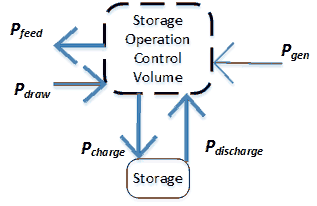
\includegraphics[width=0.9\textwidth, height=0.9\textheight, keepaspectratio=true]{media/StorageOperationControlVolume.png}
\caption{Storage operation control volume \protect \label{fig:storage-operation-control-volume}}
\end{figure}

  $ {P_{gen}}  $  This is the sum of electric power produced by the generators on the load center entering the control volume.  The generator operation is run before the storage operation so that this value is current at the time the storage operation control is evaluated 

  $ {P_{feed}}  $  This is the flow of electric power out of the control volume feeding toward the main panel.  This is power being supplied by the generators and storage and serving the building loads or perhaps being exported.  This power level might be reduced by power conversion losses before it reaches the main panel.  The method used to determine $ {P_{feed}}  $ depends on the operation scheme.
  
  $ {P_{draw}}  $  This is the flow of electric power into the control volume drawing from the main panel.  This is power being drawn in order to charge storage as desired by the storage operation scheme.  This power level might be increased by power conversion losses once it is drawn from the main panel.  

  $ {P_{charge}}  $  This is the flow of electric power into the storage device from the control volume.  This is power being supplied by the generators and/or drawn from the main panel and then directed into storage to charge the device.

  $ {P_{discharge}}  $  This is the flow of electric power out of the storage device into the control volume.  This power is being pulled from storage and added to the power from generators to feed toward the main panel. 

The **TrackFacilityElectricDemandStoreExcessOnSite** method tries to run the storage to follow the facility electric demand while storing any excess on-site power production that is above what is needed to run the facility.  This is mainly appropriate for island operation.  This is the intended legacy behavior before version 8.5.  This scheme does not draw from the main panel to charge, so we have  $ {P_{draw}} = 0.0  $.  The value for $ {P_{feed}}  $ is determined from the whole-facility total electric power demand.  (When there is more than one load center in the model, it is actually the portion of the total that remains after previous load centers have been simulated.)  This requested feed in rate is adjusted to be increased by any power conversion losses that may occur in an inverter or a transformer.  This adjusted feed in request is used for $ {P_{feed}}  $. 

If $ {P_{gen}} > {P_{feed}} $ ,  then we have charging, 

\begin{equation}
  \begin{array}{rl}
    {P_{charge}} &= {P_{gen}} - {P_{feed}} \\
    {P_{discharge}} &= 0.0
  \end{array}
\end{equation}

If $ {P_{gen}} < {P_{feed}} $ , then we have discharging

\begin{equation}
  \begin{array}{rl}
    {P_{discharge}} &=  {P_{feed}} - {P_{gen}} \\
    {P_{charge}} &= 0.0
  \end{array}
\end{equation}

The **TrackMeterDemandStoreExcessOnSite** method is very similar to the TrackFacilityElectricDemandStoreExcessOnSite method except that instead of using the whole-facility total electric demand, the value for $ {P_{feed}}  $ is determined from a user-specified meter.  The same charge and discharge logic is used. 

The **TrackChargeDischargeSchedules** method tries to run the storage to follow user-defined schedules and design power levels for charging and discharging.  The user inputs a design charge rate $ {P_{charge,design}} $, a charge modification schedule $ {f_{sched,charge}} $, a design discharge rate $ {P_{discharge,design}} $, and a discharge modification schedule $ {f_{sched,discharge}} $.  The scheduled power flows will be used to determine charging and discharging as long as other limits on rates or state of charge are not triggered.  The schedules should be arranged to only charge or only discharge at a given time.  

If charging, we have  

\begin{equation}
  \begin{array}{rl}
    {P_{charge}} &= {P_{charge,design}} * {f_{sched,charge}} \\
    {P_{discharge}} &= 0.0
  \end{array}
\end{equation}

If $ {P_{gen}} > {P_{charge}} $,  then we have excess to feed toward main panel,

\begin{equation}
  \begin{array}{rl}
    {P_{feed}} &= {P_{gen}} - {P_{charge}} \\
    {P_{draw}} &= 0.0
  \end{array}
\end{equation}

If $ {P_{gen}} < {P_{charge}} $, the we have a shortfall and we draw from main panel,

\begin{equation}
  \begin{array}{rl}
    {P_{draw}} &= {P_{charge}} - {P_{gen}} \\
    {P_{feed}} &= 0.0
  \end{array}
\end{equation}

If discharging, we have 

\begin{equation}
  \begin{array}{rl}
    {P_{discharge}} &= {P_{discharge,design}} * {f_{sched,discharge}} \\
    {P_{charge}} &= 0.0 \\
    {P_{feed}} &= {P_{discharge}} + {P_{gen}} \\
    {P_{draw}} &= 0.0
  \end{array}
\end{equation}

The **FacilityDemandLeveling** method tries to run the storage to follow a user-defined schedule for the net purchased power, $ {P_{net,purch}}  $.  This is similar to demand limit operation but instead of just attempting to cap the facility demand, it will also manipulate storage to increase utility grid supply electric to meet the target for net purchased power.  The user inputs a design demand target for net purchase power rate, $ {P_{net,purch,design}}  $, and a demand level modification schedule $ {f_{sched,dmd,target}} $.  

\begin{equation}
  {P_{net,purch,target}} = {P_{net,purch,design}} *{f_{sched,dmd,target}}
\end{equation}

This target is compared to an adjusted feed in request, $ {P_{feed, request}}  $, from the (remaining, adjusted) whole-facility total electric power demand. 

\begin{equation}
  {P_{feed}} = {P_{feed,request}} - {P_{net,purch,target}}
\end{equation}

If $ {P_{feed}} > 0.0 $, then we have a situation where the facility needs more power that the target demand.  We therefore feed that power toward the main panel, but it is not necessarily the full power request that could be served.  If $ {P_{gen}} < {P_{feed}} $, then we still have some power supply to make up by discharging,

\begin{equation}
  \begin{array}{rl}
    {P_{discharge}} &=  {P_{feed}} - {P_{gen}} \\
    {P_{charge}} &= 0.0
  \end{array}
\end{equation}

Or if $ {P_{gen}} > {P_{feed}} $,  then we have excess power we can use for charging.

\begin{equation}
  \begin{array}{rl}
    {P_{charge}} &= {P_{gen}} - {P_{feed}} \\
    {P_{discharge}} &= 0.0
  \end{array}
\end{equation}

However, if $ {P_{feed}} < 0.0 $, then the facility needs less power than the target demand.  We therefore draw power from the main panel to increase power purchased to meet target demand level. 

\begin{equation}
  \begin{array}{rl}
   {P_{draw}} &= { abs( {P_{feed}} )} \\
    {P_{feed}} &= 0.0 \\
    {P_{charge}} &= {P_{draw}} + {P_{gen}}
  \end{array}
\end{equation}

\subsection{Electrical Storage - Simple Energy Balance Model}

EnergyPlus includes two models for storing electrical energy: a simple model that is not intended to represent any specific type of storage technology and a battery model that represents the kinetic battery model originally developed by Manwell and McGowan which discussed in the next section.

The simple model treats the battery as a black box, counting energy added and removed, with losses due to charge/discharge inefficiencies. The model is a reasonable starting point for simulation of Li-ion and other battery technologies without significant rate limitations. The simple model might be called constrained bucket with energy losses.  The bucket holds a quantity of Joules of electrical energy, referred to as the state of charge. There are losses and limits to storing and drawing power but otherwise the bucket just holds electricity. The user sets constraints on the rates of charging, ${P_{stor - {\rm{charge - max}}}}$, and drawing, ${P_{stor - {\rm{d}}raw{\rm{ - max}}}}$. The user defines efficiency values for charging, ${\varepsilon_{{\rm{charge}}}}$, and drawing, ${\varepsilon_{draw}}$. 

The user defines an initial state of charge and a maximum state of charge. The storage operation scheme makes supervisory control decisions and determines a value for the charging power, ${P_{stor - ch\arg e}}$, or the discharging power, ${P_{stor - draw}}$ and passes in control limits for the minimum and maximum state of charge fraction.  The maximum state of charge is the physical capacity of the storage device, however the storage control applies a separate layer of minimum and maximum state of charge used to model controller behavior designed to protect the battery from abuse. 

The control requests are constrained by the device's physical limits for how fast it can be charged or discharged, ${P_{stor - {\rm{charge - max}}}}$ and ${P_{stor - {\rm{d}}raw{\rm{ - max}}}}$ are applied.

If charging, the new state of charge, \(Q_{stor}^{t + \Delta t}\) , is determined using:

\begin{equation}
Q_{stor}^{t + \Delta t} = Q_{stor}^t + {P_{stor - ch\arg e}} \cdot {\varepsilon_{{\rm{charge}}}} \cdot \Delta t
\end{equation}

If drawing, the new state of charge is:

\begin{equation}
Q_{stor}^{t + \Delta t} = Q_{stor}^t - \frac{{{P_{stor - draw}} \cdot \Delta t}}{{{\varepsilon_{draw}}}}
\end{equation}

Where \(\Delta t\) ~is the length of the system time step in seconds.

The storage device has an availability schedule. If it is not available then no power can be drawn or stored.  The state of charge minimum and maximum that are passed into the storage model are used to decide if the device can be further charged or discharged.  The separate control limits allow modeling battery preservation strategies where the full capacity of the storage device is not really used. 

The gross electric power drawn and stored includes losses in the form of heat. These thermal losses are calculated from the user-specified efficiencies for charging and drawing and gross electric power stored and drawn. The thermal (heat) losses are included in a zone heat balance if the user specifies a thermal zone. A user-defined radiative split is used to divide thermal losses into radiation and convection portions. If no zone is specified, then the thermal losses are simply disregarded (e.g., rejected to outdoors and do not impact the zone air heat balance).

\subsection{Electrical Storage -- Kinetic Battery Model with Cycle Life Estimation}\label{electrical-storage-kinetic-battery-model}

The Kinetic Battery Model (KiBaM) (object: ElectricLoadCenter:Storage:Battery) was originally developed by Manwell and McGowan (1993) for use in time series performance models of hybrid energy systems. The model is called kinetic because it is based on a chemical kinetics process to simulate the battery charging and discharging behavior. The model, with different improvements and modifications, has been incorporated into the software Hybrid2 and HOMER as the electrical storage module of hybrid and distributed power systems. In 2005, KiBaM was implemented as a stand-alone application in support of the European Union Benchmarking research project (Bindner et al. 2005). The model is intended to represent technologies such as Pb-acid that encounter significant rate or kinetic limitations.

The Kinetic Battery Model assumes that the battery charge is distributed over two tanks: an available-charge tank and a bound-charge tank. The tank for available charges can supply electrons directly to the load, whereas the tank for chemically bound charges can only supply electrons to the available-charge tank. At any time, the total charge \(q\) ~in the battery is the sum of the available charge (\({q_1}\) ) and bound charge (\({q_2}\) ). That is:

\begin{equation}
q = {q_1} + {q_2}
\end{equation}

Based on the governing equations on the change of charge in both tanks (Manwell and McGowan 1993), the battery capacity can be related to a constant charge/discharge current (\(I\) ) as the following equation:

\begin{equation}
{q_{\max }}(I) = \frac{{{q_{\max }}k \cdot c \cdot t}}{{1 - {e^{ - kt}} + c(kt - 1 + {e^{ - kt}})}}
\end{equation}

where,

\({q_{\max }}(I)\) ~ : Maximum capacity (Ah) at charge or discharge current I

\({q_{\max }}\) ~~~~~~ : Maximum capacity (Ah) at infinitesimal current

\(t\) ~~~~~~~~~~~ : Charge or discharge time (hr), defined by \(t = \frac{{{q_{\max }}(I)}}{I}\)

\(k\) ~~~~~~~~~~ : Constant coefficient (hr\(^{-1}\))

\(c\) ~~~~~~~~~~ : Parameter indicating the ratio of available charge capacity to total capacity

Assuming that a constant current is used in any time step for charging and discharging, the available charge (\({q_1}\) ) and bound charge (\({q_2}\) ) at any time step are given by:

\begin{equation}
{q_1} = {q_{1,0}}{e^{ - k\Delta t}} + \frac{{({q_0}kc - I)(1 - {e^{ - k\Delta t}})}}{k} - \frac{{Ic(k\Delta t - 1 + {e^{ - k\Delta t}})}}{k}
\end{equation}

\begin{equation}
{q_2} = {q_{2,0}}{e^{ - k\Delta t}} + {q_0}(1 - c)(1 - {e^{ - k\Delta t}}) - \frac{{I(1 - c)(k\Delta t - 1 + {e^{ - k\Delta t}})}}{k}
\end{equation}

where,

\({q_{1,0}}\) ~ :~ Available charge at the beginning of time step (Ah)

\({q_{2,0}}\) ~:~ Bound charge at the beginning of time step (Ah)

\({q_0}\) ~~ :~ Total charge at the beginning of time step (Ah), \({q_0} = {q_{1,0}} + {q_{2,0}}\)

\(\Delta t\) ~~ :~ Length of time step (hr)

KiBaM views the battery as a voltage source in series with an electric resistance (Figure~\ref{fig:electrical-equivalent-model-for-kibam}). The internal resistance is assumed to be constant and the open circuit voltage varies with current and state of charge.

\begin{figure}[hbtp] % fig 338
\centering

\includegraphics[width=0.9\textwidth, height=0.9\textheight, keepaspectratio=true]{media/image7528.svg.png}
\caption{Electrical equivalent model for KiBaM \protect \label{fig:electrical-equivalent-model-for-kibam}}
\end{figure}

The battery's open circuit voltage is modeled in the same form for charging and discharging, but with different coefficients. The open circuit voltage in charging (\({E_c}\) ) and in discharging (\({E_d}\) ) can be respectively expressed as:

\begin{equation}
{E_c} = {E_{0,d}} + {A_c}{X_c} + \frac{{{C_c}{X_c}}}{{{D_c} - {X_c}}}
\end{equation}

\begin{equation}
{E_d} = {E_{0,c}} + {A_d}{X_d} + \frac{{{C_d}{X_d}}}{{{D_d} - {X_d}}}
\end{equation}

where,

\({E_{0,c}}\) ~~~~~~~~~~~~~~ : Open circuit voltage for a fully charged battery

\({E_{0,d}}\) ~~~~~~~~~~~~~~ : Open circuit voltage for a fully discharged battery

\({A_c}\) , \({C_c}\) , \({D_c}\) ~~~: Constant parameters for charging

\({A_d}\) , \({C_d}\) , \({D_d}\) ~~: Constant parameters for discharging

\({X_c}\) , \({X_d}\) ~~~~~~~~: Normalized maximum capacity at a given charging or discharging current, calculated as:

\begin{equation}
X = \left\{
    \begin{array}{cl}
      q_0 / q_{max}(I) & \; (charging) \\
      (q_{max}-q_0)/q_{max}(I) & \; (discharging)
    \end{array}
  \right.
\end{equation}

It needs to be noted that the performance curve (Curve:RectangularHyperbola2) used in the model input covers the 2\(^{nd}\) and the 3\(^{rd}\) item of the open circuit voltage equation. Due to the reformatting of performance curve, the voltage function regression coefficients can map to the curve coefficients as follows:

\({C_1} = - C\) ~;\({C_2} = - D\) ;\({C_3} = A\)

With open circuit voltage, the battery terminal voltage (V) can be calculated as:

\begin{equation}
V = E - IR
\end{equation}

where, R is the battery internal resistance in Ohms; the current is positive for discharging and negative for charging.

Given desired power in/out of the battery, the desired charge or discharge current can be calculated from the basic power equation: \(P = VI\) . In this calculation, iteration is needed to ensure the electric current has converged and the battery operation satisfies all specified technical constraints such as maximum discharge current and charge rate limit.

KiBaM assumes that battery life is a primary function of charge/discharge cycles. One cycle is defined as the process of starting from a certain state of charge (SOC), the battery is discharged to a lower SOC and then recharged back to the starting SOC. It is regarded that the magnitude of cycle plays more important than the average of SOC during the cycle. This means that in terms of the impact on battery life, the cycle from 90\% to 70\% and then recharge back to 90\% of SOC is equivalent to another cycle from 50\% to 30\% and then recharge back to 50\% of SOC.~ Battery life in terms of the number of cycles is predicted as a function of the cycle range measured by the fractional depth of discharge. A double exponential equation is used to capture the damage to batteries due to cycling. The equation takes the following form where the coefficients need to be derived from battery test data via curve fitting.

\begin{equation}
{C_F} = {C_1} + {C_2}{e^{{C_3}R}} + {C_4}{e^{{C_5}R}}
\end{equation}

where,

\({C_F}\) ~~~ :~~~ Cycles to failure

\({C_1}\) -\({C_5}\) :~~~ Regression coefficients

R~~~~~~ :~~~ Cycle range in terms of fractional SOC

Following Hybrid2, the rainflow counting method (Downing and Socie 1982) is used to count battery cycles within a state of charge time series. Based on the number of cycles for each fractional SOC range, the battery damage is estimated as:

\begin{equation}
D = \sum\limits_{i = 1}^{} {\left( {{N_i}\frac{1}{{{C_{F,i}}}}} \right)}
\end{equation}

where,

D~~~ : Fractional battery damage. For example, a value of 0.5 at the end of simulation means that half of the battery life is used up after the length of the simulation period.

\({C_{F,i}}\) : Number of cycles to failure for the i-th cycle range

\({N_i}\) ~ : Total number of cycles over the simulation with the i-th cycle range

It needs to be noted that the temperature effects on battery performance and battery self-discharge are not supported in the current model.

\subsubsection{References}\label{references-021}

Bindner H., Cronin T., Lundsager P., Manwell J.F., Abdulwahid U., and Baring-Gould I. 2005. Lifetime Modeling of Lead Acid Batteries. Riso National Laboratory, Roskilde, Denmark.

Downing S. D. and Socie D. F. 1982.~ Simple rainflow counting algorithms, International Journal of Fatigue, 1982.

Manwell J. F. and McGowan J. G. 1993. A lead acid battery storage model for hybrid energy systems, Solar Energy 50(5): 399- 405.

\subsection{Electric Load Center Transformers}\label{electric-load-center-transformers}

Transformers (object name: ElectricLoadCenter:Transformer) are an integral part of the electric distribution system. They have two broad applications closely related to building energy simulation. First, transformers are used to lower the voltage of electricity from utility primary circuits to customer secondary circuits, and in this case they are called distribution transformers. Second, transformers are used to output the surplus power from onsite generators to the electricity grid.

Distribution transformers reduce the voltage on utility distribution lines (34.5 kV or less) to a lower secondary voltage (600 V or less) suitable for customer equipment. Distribution transformers are usually categorized according to the medium used for cooling and insulation (liquid or air), the voltage class that they serve (low or medium), and the number of phases (single phase or three phase).

Liquid-immersed transformers rely on oil or other fire resistant liquid around the coils for cooling. In contrast, dry type transformers rely only on the natural convection of air for insulation and cooling. Medium-voltage transformers step from utility line voltage down to a lower secondary voltage, depending on the application. The secondary voltage from a medium-voltage transformer is usually at 277 V for single phase and 480 V for three phase. This secondary voltage can be directly used as 480 V three-phase power for large motors or as 277 V single-phase power for some fluorescent lighting. However, for most industrial and commercial facilities, low-voltage transformers are needed to reduce the above voltages further to 208/120 V. Common 120 V loads are wall plugs and incandescent lighting.

Most liquid-immersed transformers are owned by utilities and they are of the medium-voltage type. Virtually all dry type transformers are owned by commercial and industrial customers (Barnes et al. 1996). Of the dry type transformers, those of the medium-voltage type are generally special-order items while those of the low-voltage type are commodity items. The efficiency requirement of distribution transformers is covered by the NEMA (National Electrical Manufactures Association) Standard TP 1. ASHRAE 90.1-2010 will cite the NEMA Standard TP 1 to stipulate the efficiency requirement for the low-voltage dry type distribution transformers.

There are two main types of energy losses in transformers: no load loss and load loss. The no load loss comes primarily from the switching of the magnetic fields in the core material. Hence, it is also called the core loss. The no load (core) loss is roughly constant and exists continuously in the core material as long as the transformer is energized. The load loss comes from the electrical resistance in the windings when there is a load on the transformer. Hence, the load loss is also called the winding loss. The load (winding) loss is proportional to the load squared with a small temperature correction.

Given the no load loss (NL) and the load loss (LL) at rated load and conditions, the total energy losses in a transformer at time t is calculated as:

\begin{equation}
TL(t) = NL + LL(t) = NL + LL*P{(t)^2}*{f_T}(t)
\end{equation}

where,

\(TL(t)\) ~~~~~~~ Total energy loss at time t (W)

\(LL(t)\) ~~~~~~~ Load loss at time t (W)

\(P(t)\) ~~~~~~~~~ Per unit load at time t

\({f_T}(t)\) ~~~~~~~~ Temperature correction factor for the load loss at time t

The per unit load at time t is calculated as:

\begin{equation}
P(t) = \frac{{Load(t)}}{{{S_B}}}
\end{equation}

where,

\(Load(t)\) Transformer load at time t (W)

\({S_B}\) Transformer nameplate rating (VA)

The temperature correction factor at time t is calculated as (NEMA 2002):

\begin{equation}
{f_T}(t) = {L_{dc}}*\frac{{R(t)}}{{{R_{ref}}}} + {L_{eddy}}*\frac{{{R_{ref}}}}{{R(t)}}
\end{equation}

where,

\({L_{dc}}\) ~~~~~~~~~~~ Per unit load loss due to electrical resistance

\({L_{eddy}}\) ~~~~~~~~~ Per unit load loss due to eddy currents

\(R(t)\) ~~~~~~~~~ Winding electrical resistance at time t

\({R_{ref}}\) ~~~~~~~~~~ Winding electrical resistance at the full load reference conditions

The ratio of winding electrical resistance is calculated as:

\begin{equation}
\frac{{R(t)}}{{{R_{ref}}}} = \frac{{F + {T_{winding}}(t) + {T_{amb}}(t)}}{{F + {T_{winding,ref}} + {T_{amb,ref}}}}
\end{equation}

where,

\(F\) ~ Thermal coefficient of resistance for the winding material ( = 225 for aluminum and 234.5 for copper)

\({T_{winding,ref}}\) Winding temperature rise at the full load reference conditions (°C)

\({T_{winding}}(t)\) Winding temperature rise at time t (°C)

\({T_{amb,ref}}\) ~~~~~~ Ambient temperature at the reference condition ( = 20 °C)

\({T_{amb}}(t)\) ~~~~~ Ambient temperature at time t (°C)

The Ambient temperature \({T_{amb}}(t)\) is equal to the zone temperature if a thermal zone is specified in the input; otherwise, it is assumed equal to 20 °C. The winding temperature rise at time t is calculated as (Barnes et al. 1997):

\begin{equation}
{T_{winding}}(t) = P{(t)^{1.6}}*{T_{winding.ref}}
\end{equation}

Based on the derived total energy losses in a transformer, the transformer efficiency at time t can be calculated according to the following equation:

\begin{equation}
\eta (t) = \frac{{Load(t)}}{{Load(t) + NL + LL(t)}}
\end{equation}

The above procedure describes how to calculate the total transformer energy losses based on the no load loss and load loss at rated conditions. The transformer model also supports the case when the nominal transformer efficiency is given. In this case, the user needs to provide the nameplate efficiency and the corresponding per unit load, the maximum efficiency and the corresponding per unit load, and the reference conductor temperature at which the nameplate efficiency is measured. Given these information, both no load loss and load loss at rated conditions can be derived as below.

The nameplate efficiency can be expressed as:

\begin{equation}
{\eta_{np}} = \frac{{{S_B}*{P_{np}}}}{{{S_B}*{P_{np}} + NL + LL*P_{np}^2*{f_{T,np}}}}
\end{equation}

where,

\({\eta_{np}}\) ~~~~~~~~~~~ Nameplate efficiency

\({S_B}\) Nameplate rating (VA)

\({P_{np}}\) ~~~~~~~~~~~ Per unit load at which the nameplate efficiency is measured

\({f_{T,np}}\) ~~~~~~~~~ Applied temperature correction factor for the nameplate efficiency

Maximum efficiency generally occurs when the load loss is equal to the no-load loss. Because the no-load loss does not vary with the load on the transformer, the following relationship can be established:

\begin{equation}
NL = L{L_{\max ,\eta }} = LL*P_{\max ,\eta }^2*{f_{T,\max  - \eta }}
\end{equation}

where,

\({P_{\max ,\eta }}\) ~~~~~~~~ Per unit load at which the maximum efficiency is obtained

\({f_{T,\max - \eta }}\) ~~~~ Applied temperature correction factor for the maximum efficiency

Transformers typically have close per unit loads for the nameplate efficiency and the maximum efficiency. Therefore, it is reasonable to assume that the applied temperature correction factors are equal at those two efficiencies. This implies that:

\begin{equation}
\frac{{L{L_{np}}}}{{L{L_{\max ,\eta }}}} = \frac{{LL*{P_{np}}^2*{f_{T,np}}}}{{LL*{P_{\max ,\eta }}^2*{f_{T,\max  - \eta }}}} = {\left( {\frac{{{P_{np}}}}{{{P_{\max ,\eta }}}}} \right)^2}
\end{equation}

Rearranging Equation and combining it with Equation leads to:

\begin{equation}
L{L_{np}} = L{L_{\max ,\eta }}*{\left( {\frac{{{P_{np}}}}{{{P_{\max ,\eta }}}}} \right)^2} = NL*{\left( {\frac{{{P_{np}}}}{{{P_{\max ,\eta }}}}} \right)^2}
\end{equation}

Combining Equations and , we can obtain the no load loss as:

\begin{equation}
NL = \frac{{{S_B}*{P_{np}}*(1 - {\eta_{np}})}}{{{\eta_{np}}*\left[ {1 + {{\left( {\frac{{{P_{ref}}}}{{P{}_{\max ,\eta }}}} \right)}^2}} \right]}}
\end{equation}

Substitute NL into Equation , we can calculate the load loss at rated conditions as:

\begin{equation}
LL = \frac{{NL}}{{{f_{T,\max  - \eta }}*P_{\max ,\eta }^2}} = \frac{{NL}}{{{f_{T,np}}*P_{\max ,\eta }^2}}
\end{equation}

Since both no load and load losses at rated conditions are known, the total energy losses in a transformer at time t can then be calculated according to Equation

\subsubsection{References:}\label{references-1-008}

Barnes, PR., JW. Van Dyke, BW. McConnell, and S. Das. 1996. Determination Analysis of Energy Conservation Standards for Distribution Transformer, ORNL-6847. Oak Ridge National Laboratory, Oak Ridge, TN.

Barnes, PR., S. Das, BW. McConnell, and JW. Van Dyke. 1997. Supplement to the ``Determination Analysis'' (ORNL-6847) and Analysis of the NEMA Efficiency Standard for Distribution Transformer, ORNL-6925. Oak Ridge National Laboratory, Oak Ridge, TN.

NEMA. 2002. NEMA Standards Publication TP 1-2002: Guide for Determining Energy Efficiency for Distribution Transformers. National Electrical Manufactures Association, Rosslyn, VA.
